\documentclass[12pt,a4paper]{article}

\usepackage[utf8]{inputenc}
\usepackage[greek,english]{babel}
\usepackage{alphabeta} 

\usepackage[pdftex]{graphicx}
\usepackage[top=1in, bottom=1in, left=1in, right=1in]{geometry}

\linespread{1.06}
\setlength{\parskip}{8pt plus2pt minus2pt}

\widowpenalty 10000
\clubpenalty 10000

\newcommand{\eat}[1]{}
\newcommand{\HRule}{\rule{\linewidth}{0.5mm}}

\usepackage[official]{eurosym}
\usepackage{enumitem}
\setlist{nolistsep,noitemsep}
\usepackage[hidelinks]{hyperref}
\usepackage{cite}
\usepackage{lipsum}
\usepackage{amsmath}


\begin{document}
	
	%===========================================================
	\begin{titlepage}
		\begin{center}
			
			% Top 
			
\includegraphics[width=0.55\textwidth]{Shanghaitech.png}~\\[2cm]
			
			% Title
			\HRule \\[0.4cm]
			{ \LARGE 
				\textbf{Project Report for CS181}\\[0.4cm]
				\emph{Practical Minimax Connect 4 AI}\\[0.4cm]
			}
			\HRule \\[1.5cm]
			
			
			
			% Author
			{ \large
				Zhixin Fang, Yijing Ren, Songhui Cao \\[0.1cm]
				AI Group 7\\[0.1cm]
				\texttt{fangzhx@shanghaitech.edu.cn}\\
				\texttt{renyj@shanghaitech.edu.cn}\\
				\texttt{caosh@shanghaitech.edu.cn}\\
			}
			
			\vfill
			
			%\textsc{\Large Cyprus University of Technology}\\[0.4cm]
			\textsc{\large School of Information Science \& Technology,\\
			ShanghaiTech University}\\[0.4cm]
			
			
			% Bottom
			{\large \today}
			
		\end{center}
	\end{titlepage}
	
	\begin{abstract}
		This project is a practical AI solution for Connect 4 Game. The game is proven to be solvable, however, due to its big state space, a perfect solver can be extremely tough for a regular computer to run.
		\\
		
		Thus, we decided to find a sub-optimal but practical solution of the game, it should win/draw most of the games against human players/random AI players/greedy AI players, while maintain a time efficiency of 500ms/step on a regular computer.
		\\
		
		The tool we use to create this game is Unity. We utilized its physical engine to run the base game loop, in order to reduce the cost of the game itself. An external asset, Connect 4 Starter Pack, made by Eikester is used, mainly for the game's element, like chess pieces and boards.\\
		
		To open the project in Unity, you need an Unity Editor. However, if you only want to play with it, the build can be played in Windows. The editor version we use is \textbf{2019.4.13f1c1},
		it can be downloaded as 2019 LTS version in Unity Hub.
		
	\end{abstract}
	
	
	\newpage
	
	\section{Introduction}
	This project is a practical AI solution for Connect 4 Game. Connect 4 is a game where two players push their pieces into the chessboard, and win whenever they connect a line of 4 pieces.
	\\
	
	The solution is based on minimax algorithm and a heuristic function. The solution itself is trivial, search through an adversary search tree, get optimal path.
	\\
	
	The main challenge of this project is optimization. The state space of this game is about $6^{42}$(Accounting action sequence, if reduced to only rational state, it's still huge at about $4*10^{16}$ states), so the complexity can be very high. We applied a few optimization techniques, namely alpha-beta pruning and transposition table, aiming to reduce the calculation time for each step to 500ms at most.
	\\
	
	\section{Division of Work}
	\begin{enumerate}
		\item [Zhixin Fang:] Game programming, Heuristic Design and Programming, Interface \& System Structure planning, Optimization design, Report \& Presentation
		\item [Yijing Ren:] Verification, Video making, Helper function implementation
		\item [Songhui Cao:] Algorithm design \& Implementation, Optimization design \& Implementation
	\end{enumerate}
	\section{How to Play}
	This section contains instructions on operating the game, and some mechanism we use to implement the game with minimum performance overhead.\\
	
	
	\subsection{Main Menu}
	\quad \\
	
	When you enter the game you will be in the main menu. You can configure two players and the heuristics they use. Parameter adjustments can be done for heuristics here as well.\\
	
	Modified data for heuristics will be stored between games, but it will be deleted upon exit.\\
	
	After you've done configuring, click start to begin the game.
	\textbf{If you run the game in Unity Editor, be sure to start at the preload scene. It is used to store data.}
	\subsection{Game Loop}
	\quad\\
	
	The game loop is not the focus of the project, only a brief introduction here will be done here. If you are curious about how the game functioning, see GameController.cs.\\
	
	The game runs as soon as you click the start button. Red(player 2) will take the first move, then Blue(player 1) follows, take turns until one side connect a 4 pieces line.\\
	
	After the game is ended(either a win or a draw), you can click on play again button to return to the main menu, and start again.\\
	
	To exit the game, you press Alt F4 just like exiting any other applications in Windows.
	
	\section{Algorithm}
	This part introduces the algorithms we use. A heuristic function, which is used to calculate utility, will also be explained.
	
	\subsection{Minimax}
	\textbf{Minimax algorithm} is the basic algorithm for adversary search. It's a perfect suit for Connect-4, since two players take turns to chase the win.\\
	
	Connect-4 is proven to be solvable, i.e. there's a specific solving strategy that a player can apply to achieve guaranteed victory, and Minimax algorithm, obviously can be that solver. However, as explained in the introduction part, even heavily optimized Minimax solver can't always resolve the game in an acceptable speed for a step(for us, it's 500ms), and an unwinnable AI is no fun to play against, hence we switched our focus to make a fast, sub-optimal, practical optimized Minimax algorithm.\\
	
	The base idea of Minimax Algorithm is unchanged, we will program max-agent and min-agent, simulate a few steps in a depth-first search tree. Max-agent will try to maximize the utility, while min-agent tries to minimize it. We won't cover the algorithm's detail here and in the implementation part, because the explanation for it is basically everywhere on the internet.\\
	
	The problem is, what's the utility in this game? It does not have any score system available like the Pacman, how should the AI decide whether a move is bad or not?
	
	\subsection{Heuristic}
	The answer we propose to the previous question, is \textbf{Heuristic Function}. It's basically a score calculator, giving the AI an idea on how the situation is.\\
	
	\subsubsection{Heuristic Parameter Design}
	After searching online we found an article, target specifically on evaluating a game field for Connect-4.\\
	
	There are 5 parameters for this heuristic - Block, Good, Win, Danger, Lose, which corresponds to 5 different type of Connect-4 lines(4 consecutive slot, we will short this term as "4-line" in the following context).\\
	
	
	\begin{enumerate}
		\item [Block:] A Block is a 4-line where there are both friendly pieces and adversary pieces. No one can win from such 4-lines. For defensive strategy, set this factor to small positive number, for aggressive strategy, set it to negative.
		\item [Good:] A 4-line with only friendly pieces is considered good for the AI. The more pieces in it, the better it is. This parameter should be a mildly big positive number.
		\item [Win:] A Win 4-line, is namely a 4-line with all friendly pieces inside. Reaching this state means victory, so the parameter for it is a generally a big positive number.
		\item [Danger:] A 4-line with only adversary pieces is considered dangerous, this parameter works just like Good factor, the more enemy pieces, the more dangerous. It should be set to a mildly big (abs) negative number.
		\item [Lose:] A 4-line fully of adversary pieces means the AI's defeat, so it should be a big (abs) negative number.
	\end{enumerate}

	Namely, each 4-line can be represented by this equation:
	\begin{displaymath}
		4 = num(empty) + num(friendly) + num(adversary)
	\end{displaymath}
	The categorize function for each line is:
	$$categ(line)=
	\begin{cases}
	Block, & num(friendly) > 0 , num(adversary) > 0\\
	Good, & num(friendly) > 0 , num(adversary) = 0\\
	Win, & num(friendly) = 4\\
	Danger, & num(friendly) = 0 , num(adversary) > 0\\
	Lose, & num(adversary) = 4
	\end{cases}
	$$

	\subsubsection{Field Categorization}
	In a typical Connect-4 field, there are 6 rows, 7 columns, so 42 slots in total. The heuristic function needs to traverse all 4-lines, namely horizontal, vertical and diagonal ones to find the score of a field.\\
	
	We divide the field to 4 types of line field correspondingly, and evaluate as follows.\\
	
	{\centering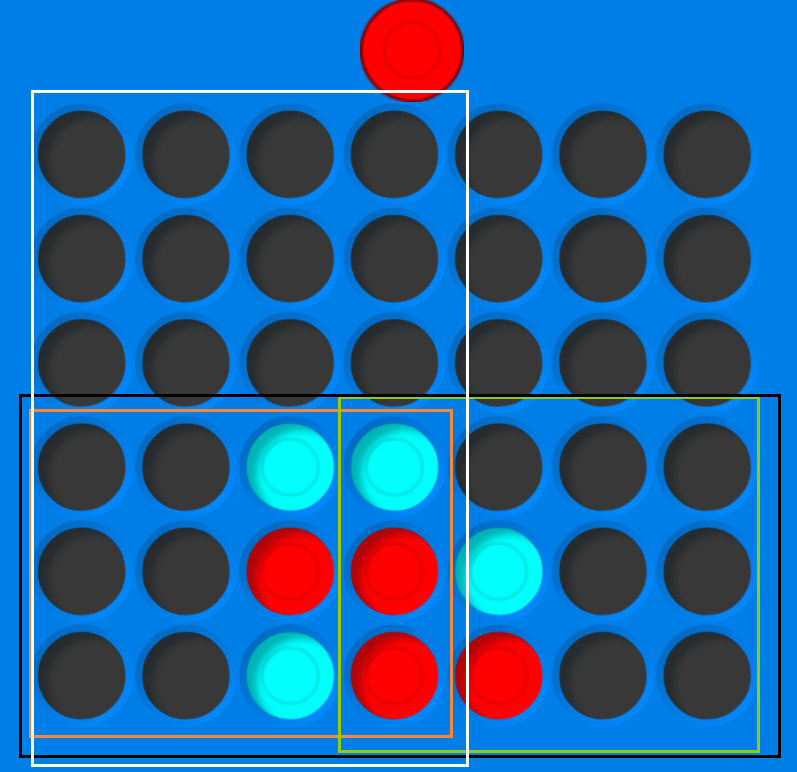
\includegraphics[width=0.5\textwidth]{LineField.png}~\\}
	
	\begin{enumerate}
		\item [White:] Horizontal Field: Includes all possible start slots for horizontal line(reaching to right)
		\item [Black:] Vertical Field: Includes all possible start slots for vertical line(reaching to upside)
		\item [Orange:] Diagonal A Field: Includes all possible start slots for diagonal line type A(reaching to upper-right)
		\item [Green:] Diagonal B Field: Includes all possible start slots for diagonal line type B(reaching to upper-left)
	\end{enumerate}

	This categorization of the game field covered all possible lines in the game, and opens up some space for optimization, which we'll discuss later.
	
	\subsubsection{Heuristic Compute Process}
	
	To get a state's utility, we need two input, namely the field(as a 2D int array) and a player number. The player number indicates the friendly color of this evaluation, so the AI player should pass its own player number in the function.
	
	The computation process is trivial, at least for now. It loops over 4 fields mentioned above, examine each 4-line it possesses, determines what type of 4-line it is, then evaluate it. The utility of the board is the sum of all its 4-lines' value.\\
	
	The evaluation function for each type of line can be represented as:
	$$value(line)=
	\begin{cases}
		BlockFactor, & categ(line) = Block\\
		GoodFactor * num(friendly), & categ(line) = Good\\
		WinFactor, & categ(line) = Win\\
		DangerFactor * num(adversary), & categ(line) = Danger\\
		LoseFactor, & categ(line) = Lose
	\end{cases}
	$$
	
	\subsection{Implementation Details}
	In this section, we talk about technical details of the project. We'll focus more on AI/Heuristic side than the game itself.
	
	\subsubsection{System Structure}
	The game is controlled by a singleton called \textbf{GameController.cs}. It take turns to ask both players for action, then drops a piece to given place. At the end of each round, it uses Ray Casting to check if one side has win the game, then continue. Raycasting utilizes the physic system of Unity, lowering the CPU resources needed for the game itself.
	
	The controller uses a 2D array as representation of the chessboard. Note that it's \textbf{column major} and \textbf{upper-left origin}, as following picture shows.
	
		{\centering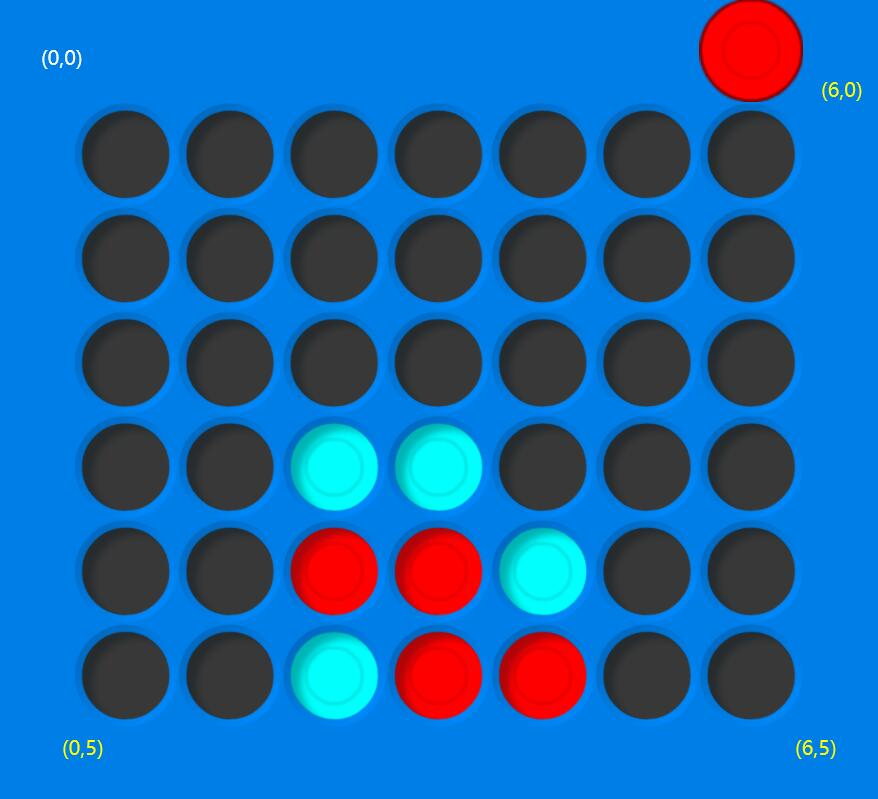
\includegraphics[width=0.5\textwidth]{Majorness}~\\}
	It also dictates a specific interface for AI script to use, which we'll describe in the next part.
	\subsubsection{AI Interface}
	The AI interface that each AI script should implement is included in \textbf{BaseAI.cs}. Apart from some public utility functions for the UI, the most important \textit{GetAction()}. The AI should extract information from the game controller, then calculate its action and return it back to the controller.
	
	The primary implementation of this interface is Minimax.cs. It has 3 typical minimax functions, namely \textit{MinimaxValue(), MinimaxMinValue(), MinimaxMaxValue()}, they respectively serve as main recursive caller, minimum node and maximum node. For more details, please check the code comments.
	
	A helper function, \textit{MinimaxAICheckWin()} is implemented for terminal state check. It takes last piece putted in the board and count to see if causes a win, i.e. causes a terminal state.
	\subsubsection{Heuristic Interface}
	Heuristic function is implemented exactly as the design suggested, but with a pruning trick for optimization(especially in early stages).
	
	\textbf{BaseHeuristic.cs} dictates interface that heuristic functions need to implement. Note that \textit{LastError} comes from a abandoned design for algorithm. All related implementations serve no purpose in the current state of the project. The core function of a heuristic is \textit{GetScoreOfBoard()}, it takes the game field and a number to calculate the utility for that player in the specified state. As you can imagine, this function will be called at terminal states to generate utility.
	
	\section{Optimization}
	After we implemented and verified the base algorithm, we discover that, as expected, the AI slows down severely after the search depth exceeds 5. To make it a far-seer, we tried a few types of optimization for the game.
	\subsection{Alpha-Beta Pruning}
	The first optimization approach we tried is Alpha-Beta pruning.\\
	
	\textbf{Max-Beta Pruning:} When a maximum node get a value, the algorithm will compare it to Beta(The current minimum available value for all minimum node from this node to root). If this value is no smaller than Beta, all of its children can be discarded. The reason for this is, maximum node only gets increasing value, but this value is already bigger than minimum available value, so it is bound to be discarded later by a minimum node. Thus, we can safely discard this node's children.
	
	\textbf{Min-Alpha Pruning:} This is a symmetric case of the Max-Beta Pruning. Minimum node only gets decreasing value, so if it already holds a value that is smaller than the current available maximum value, it is bound to be discarded later by a maximum node. Similarly, we discard its children.
	
	This optimization results in a huge leap of computation speed, it's very fast when search depth is limited to 7-8.
	\subsection{Heuristic Pruning}
	Since empty 4-line makes no contribution to the heuristic value, we can prune some positions that are bound to be empty according to physics. We prune those 4-lines' start point using the following strategy.\\
	
	{\centering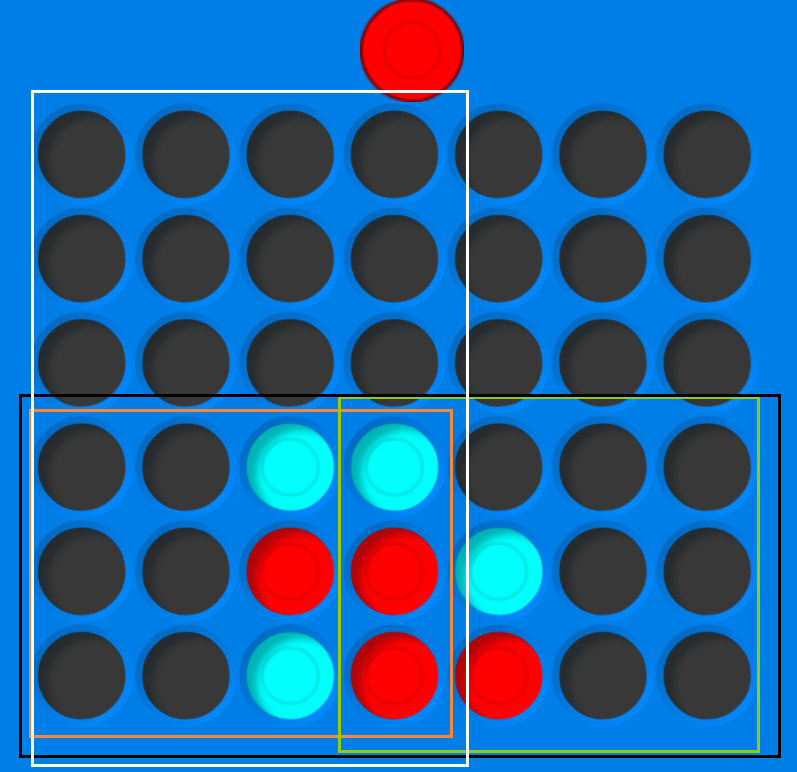
\includegraphics[width=0.5\textwidth]{LineField.png}~\\}
	
	\begin{enumerate}
		\item [Horizontal:] If a slot is empty, then all lines above it must be empty.
		\item [Vertical:] All-empty vertical lines' start point must have all empty start points above it.
		\item [Diagonal A:] Same as Vertical.
		\item [Diagonal B:] Same as Vertical
	\end{enumerate}

	This optimization affects higher search depth since more terminal states present. The improvement is minor.
	\subsection{State Cache}
	Yearning for getting more search depth, we decided to deploy a cache-like data structure to try shrink the state space.\\
	
	The thing is, although approach in different action sequence, some states are basically the same, for example, in the search tree of first 4 rounds, the action sequence 1-3-2-4 is basically the same as 2-4-1-3, because they both cause the same state of the following picture:
	\\
	
	{\centering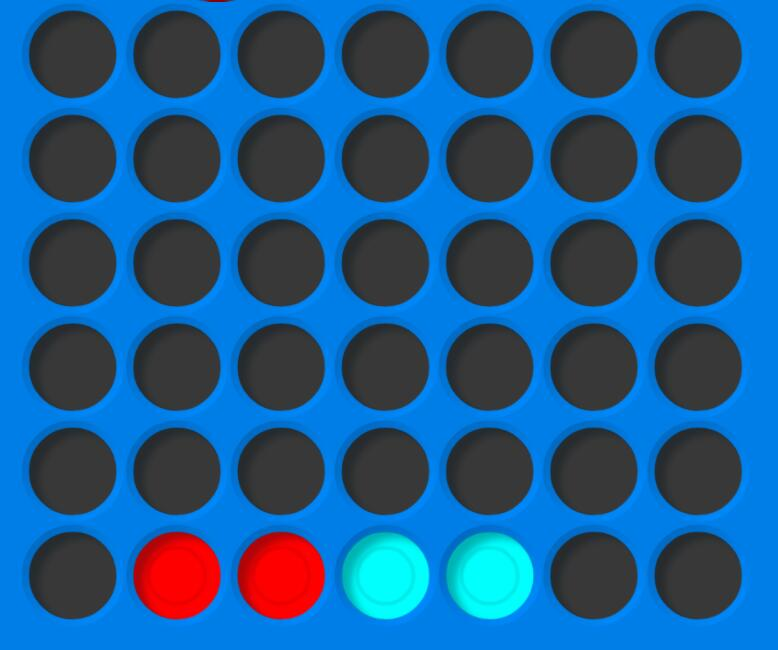
\includegraphics[width=0.5\textwidth]{Field}~\\}
	
	What's more, the field, as a 6*7 int array, is perfectly hashable. Thus, we decided to deploy a cache-like hash table for storing the state score. Once a state is in the cache, all it's children can be discarded, provide the cached value is obtained in the same depth.\\
	
	We spent a lot of time try to design a balanced cache to lower the miss cost. At last, we decided to divide the cache into 7 groups, marked by the \textbf{filled highest column} of the field state. This way, states in the different cache groups should be approximately balanced.\\
	
	The way we use the cache is trivial, before checking successors for each state, first see if it's in the corresponding cache group. If it is, we directly return the cached value, discard all its children, because a cache hit indicates we've already walked through this state before, a different action sequence does not make any difference in utility.\\
	
	The outcome of this optimization is minor in lower search depth, noticeable in higher depth like the upper-bound we give(11). We decide that the acceptable maximum search depth is 9.
	
	
	\newpage
	\section{Verification and Results}
	\subsection{Verification}
	We performed some pre-build verification when the development is not yet finished. You can still perform them in the unity editor, but since the build verification is based on the correctness of them, passing build verification will mean passing pre-build verification.
	
	{\centering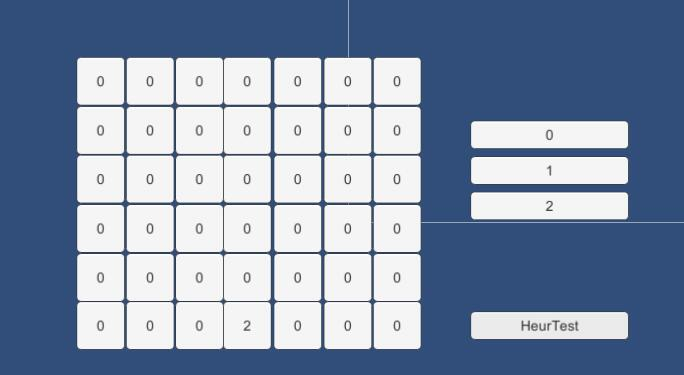
\includegraphics[width=0.5\textwidth]{Test}~\\}
	\subsubsection{Pre-build Correctness Verification}
	\begin{enumerate}
		\item [Terminal Check:] Verification for terminal state check function can be done in the \textit{Test} Scene. In this scene, you click the play button to initialize testing, then \textbf{click the 0/1/2 button on the right side} to choose which type of chesspiece you want to put in the board.\\
		In this part, you may not abide the rule of physics and the rule of the game. For each modification you make on the board, a debug log will appear on the console to show if this step made the board into terminal state. \textbf{It should output "Yes" whenever the change made a filled 4-line}.\\
		
		\item [Heuristic Prune:] This verification can be set up the same way as Terminal Check, however, this time you must construct a physically legitimate board, and click \textit{HeurTest} button. It will calculate a correct heuristic value(without pruning) using the selected heuristic function's factor. If the no-prune value is the same as the one selected function outputs, you pass the test.\\
		
		\item [Minimax:] We test the correctness of Minimax algorithm in a different way. Before we did optimization stuff, a greedy AI, \textbf{OneStepMinimaxAi.cs} was implemented first for reference. To test the correctness, we ran this AI with 1-depth minimax AI to see if their behavior is consistently similar. We delete it from the build since it's basically the same as 1-depth minimax.
	\end{enumerate}
	\subsubsection{Build Correctness Verification}
	Post-Build tests are simple, because it's only for the optimizations. A correct optimization should result in same behavior as non-optimized version of the algorithm, but with higher speed.
	\begin{enumerate}
		\item [Alpha-Beta:] Run MinimaxPruning against Minimax at depth 5, using same heuristic settings. Consistently similar behavior should be observed.
		\item [Cache:] Run MinimaxPruning against CachedMinimax at depth 9, using same heuristic settings. Consistently similar behavior should be observed.
	\end{enumerate}

	\subsection{Result}
	All Tests passed.\\
	
	The crew members also tried to have some fun with the AI we created together. We discovered the fact that, the performance of the AI is highly dependent on heuristic settings. A well tuned heuristic is barely winnable for humans, since human often can't simulate the game for 10+ steps. However, bad parameters could result in AI making confusing moves, if we tune the good factor to negative, we can create an AI that deliberately loses. We can even randomly generate parameters to make it more interesting in the future.\\
	
	At this point, it's safe to say we've created a practical AI solution for the Connect-4 game.
	\pagebreak
	\section{External Sources}
	It's safe to say that we created this project completely by ourselves! Although it's simple it consumed a hell lot of time for three of us.
	\subsection{Connect 4 Starter Pack}
	\url{https://assetstore.unity.com/packages/templates/connect-four-starter-kit-19722}\\
	
	Author: Eikester\\
	
	We used this starter kit purely for graphical element. The game logic and project structure are almost completely different.
	
	\subsection{Code Bullet Video}
	\url{https://www.youtube.com/watch?v=XRVA5PMSKKE}
	
	Author: Code Bullet\\
	
	An entertaining video that we occasionally found on the internet, serving as our inspiration. It's of almost no technical contents though, just a pure laugh matter.
	

	
	
\end{document} 
